\titledquestion{Triangelns vinkelsumma}
Denna vecka ska vi öva på att föra geometriska resonemang. Uppgifterna kommer endast att kräva det som står under ''Vinklar'' på formelbladet. 

En linje ritas genom ett av hörnen på en triangel så att linjen är parallel med motstående sida. Se figur 1.

\begin{figure}[H]
    \centering
    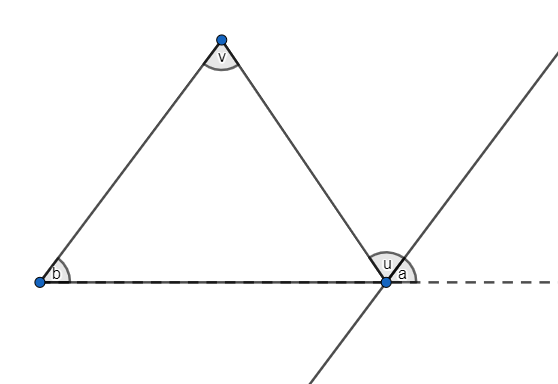
\includegraphics[width=0.5\linewidth]{img/prop32.png}
    \caption{}
\end{figure}

\begin{parts}
  \part Visa att vinklarna $a$ och $b$ är lika stora.
  \part Visa att vinklarna $v$ och $u$ är lika stora.
  \part Visa att triangelns vinkelsumma är \ang{180}.
  \part Visa att yttervinkeln i en triangel är lika med summan av de två motstående innervinklarna. 
\end{parts}


\titledquestion{Vinklar i ett parallellogram}
En parallellogram är en fyrhörning där motstående sidor är parallella.

\begin{parts}
  \part Visa att motstående vinklar i en parallellogram är lika stora.
  \part[\het] Visa att om motstående vinklar i en fyrhörning är lika stora så är fyrhörningen en parallellogram.
\end{parts}